In this work, we develop our generalized hierarchical Bayesian modeling framework that is able to capture the hierarchical structural relations and latent relations in the real-world recommendation scenarios. In our framework, we incorporate both user specific features and user events into model learning so that more personalized recommendation results can be achieved. Furthermore, we present a variational inference algorithm for the HBayes framework to provide fast parameter estimation.

In the following, we will describe how HBayes works by using apparel recommendation as an illustrative example. Using a real-world example helps explain the latent variables, hierarchy structural relations, and the conditional independence assumptions implied in HBayes. Please note that even we explain HBayes in apparel recommendation, the framework itself can be generalized into other recommendation scenarios with little modification. 



\subsection{Generative Process}

In the real-world scenario, each item or product has to come with a brand and a brand may have more than one items in the hierarchical structures. Therefore, we denote each event $t$ as a 4-tuple (Item, Brand, User, IsClick), i.e, ($\mathbf{X}_t, b_t, u_t, y_t$). $\mathbf{X}_t$ represents the item features associated with event $t$ and $y_t$ is the binary label that indicates whether user $u_t$ has clicked $\mathbf{X}_t$ or not. $b_t$ is the brand of item $\mathbf{X}_t$. 

Furthermore, we expand the hierarchy by a hidden factor, i.e., ``style''. Products from each brand $b_t$ tend to exhibit different styles or tastes, which are unknown but exist. In this paper, brands are represented as random mixtures over latent styles, where each style is characterized by a distribution over all the items. Let $S$, $B$, $U$ and $N$ be the total number of styles, brands, users and events.

The generative process of HBayes can be described as follows:

\begin{enumerate}
\item[Step 1.] Draw a multivariate Gaussian prior for each user $k$, i.e, $\mathbf{U}_k \sim \mathcal{N}(\mathbf{0}, \delta_u^{-1}\mathbf{I})$ where $k \in \{1, \cdots, U\}$.

\item[Step 2.] Draw a multivariate Gaussian prior for each style $j$, i.e, $\mathbf{S}_j \sim \mathcal{N}(\mathbf{w}, \delta_s^{-1}\mathbf{I})$ where $j \in \{1, \cdots, S\}$.

\item[Step 3.] Draw a style proportion distribution $\boldsymbol{\theta}$ for each brand $i$, $\boldsymbol{\theta} \sim \mbox{Dir}(\boldsymbol{\gamma})$  where $i \in \{1, \cdots, B\}$.

\item[Step 4.] For each brand $i$:
	\begin{enumerate}
		\item[Step 4.1] Draw style assignment $\mathbf{z}_i$ for brand $i$ where the selected style $p$ is sampled from $\mbox{Mult}(\boldsymbol{\theta})$. $\mathbf{z}_i$ is a $S\times1$ one hot encoding vector that $z_{i,p} = 1$ and $z_{i,j} = 0$ for $j = 1, \cdots, p-1, p+1, \cdots, S$.
		\item[Step 4.2] Draw $\mathbf{B}_i \sim \mathcal{N}(\mathbf{S}_{p}, \delta_b^{-1}\mathbf{I})$.
	\end{enumerate}

\item[Step 5.] For each event $t$, draw $y_t$ from Bernoulli distribution where the probability $p$ is defined as $p(y_t|\mathbf{x}_t, \mathbf{B}_{b_t}, \mathbf{U}_{u_t})$.
\end{enumerate}

\noindent where $\delta_s$, $\delta_u$ and $\delta_b$ are the scalar precision parameters and $\mathbf{w}$ is the prior mean of $\mathbf{S}_j$. 

In this work, in order to have the higher modeling flexibility and capacity, we also treat each distribution's parameter as a random variable and define hyper-priors over them. More specifically, We draw the prior mean $\mathbf{w}$ from $\mathcal{N}(\mathbf{0}, \delta_w^{-1}\mathbf{I})$. For $\delta_w$, $\delta_s$, $\delta_u$ and $\delta_b$, we define Gamma priors over them i.e.,  $p(\delta_*) = \mathcal{G}(\alpha, \beta)$, where $\delta_* \in \{ \delta_w, \delta_s, \delta_u, \delta_b \}$. 

The family of probability distributions corresponding to this generative process is depicted as a graphical model in Figure \ref{fig:model}.

\begin{figure}[htb]
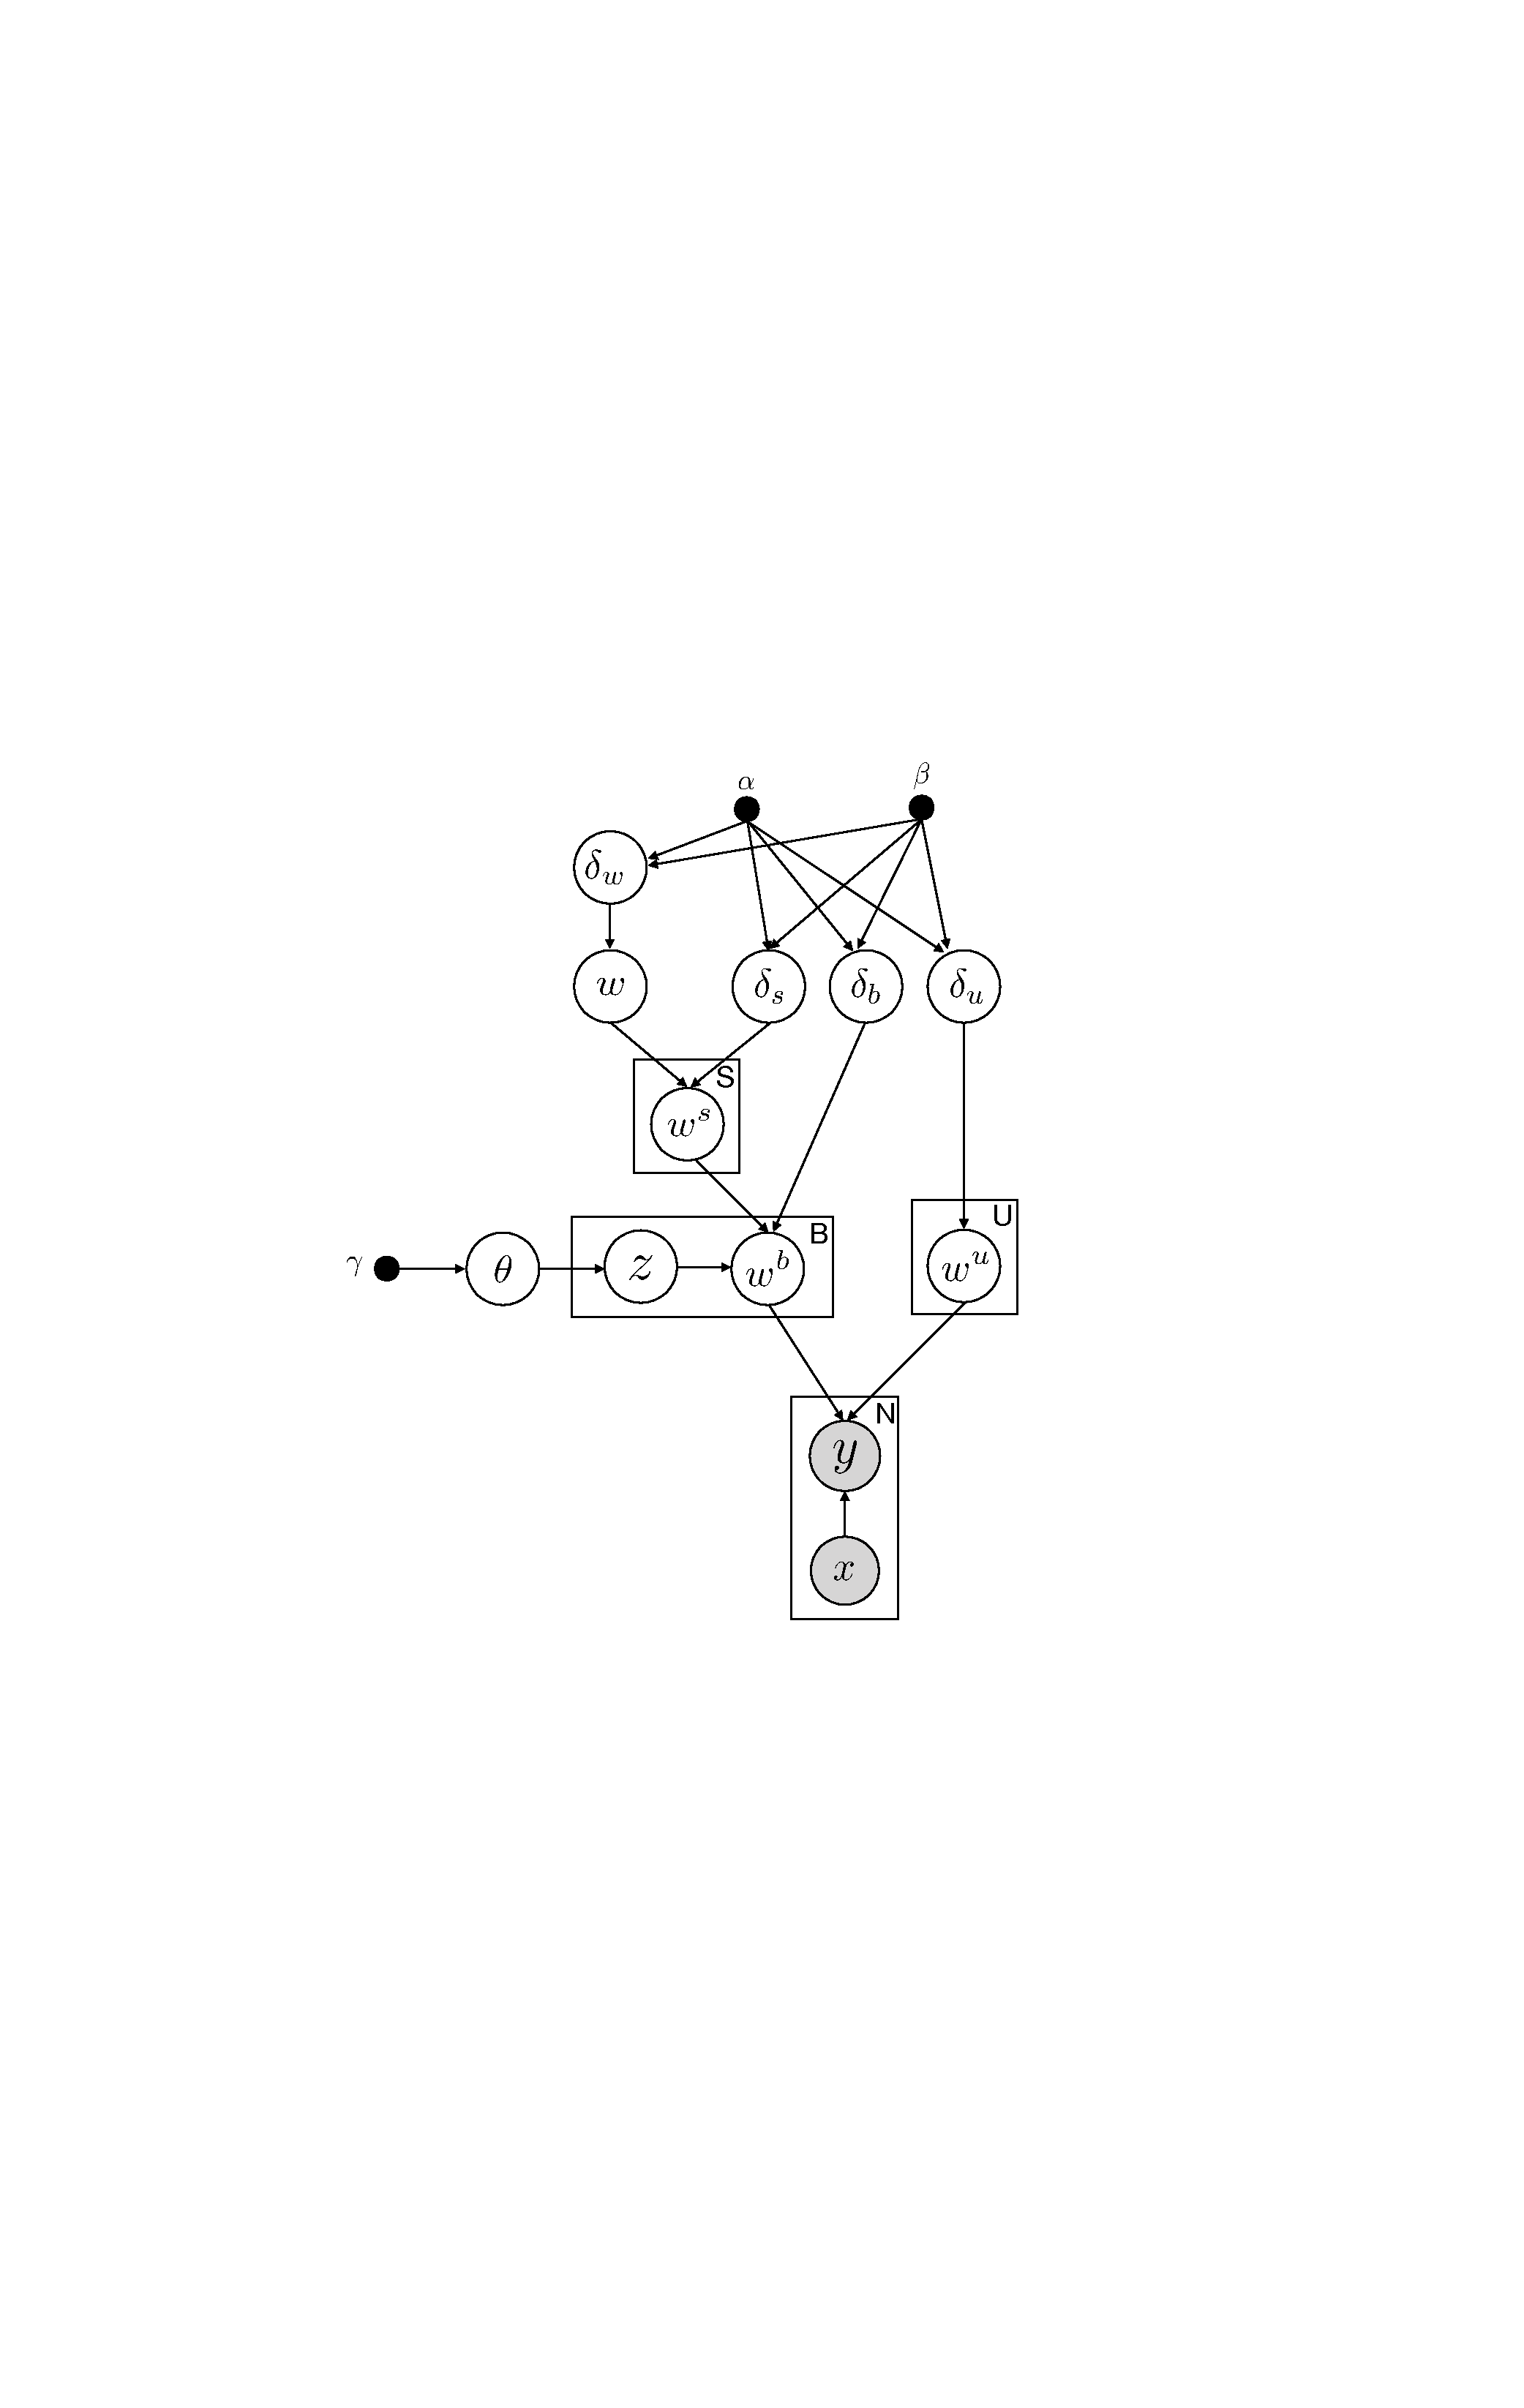
\includegraphics[width=0.8\linewidth]{fig/model}
\caption{A graphical model representation of HBayes.}
\label{fig:model}
\end{figure}

\subsection{Probability Priors \& Models}

In this work, we model the probability of a single event $t$ given ($\mathbf{X}_t, b_t, u_t, y_t$) as 

\begin{equation}
\label{eq:sigmoid_prob}
p\big(y_t|\bm{X}_t,\bm{B}_{b_t},\bm{U}_{u_t} \big)= \Big[\sigma\big(h_t\big)\Big]^{y_t} \cdot \Big[1-\sigma\big(h_t\big)\Big]^{1-y_t}
\end{equation}

\noindent where $\sigma(\cdot)$ is a logistic function, i.e. $\sigma(x)=(1+e^{-x})^{-1}$. $h_{t}=\bm{X}_t^T(\bm{B}_{b_t}+\bm{U}_{u_t})$. $\mathbf{X}^T$ is the vector transpose of $\mathbf{X}$. $\bm{U}_{u_t}$ represents user specific information encoded in HBayes for user $u_t$ and $\bm{B}_{b_t}$ denotes the brand $b_t$'s specific information.

As mentioned in Step 3 of the generative process of HBayes, each brand $i$'s style proportion distribution $\boldsymbol{\theta}$ follows a Dirichlet distribution: $p(\boldsymbol{\theta}) \sim Dir(\boldsymbol{\gamma})$, which is defined as follows: 

\begin{equation*}
Dir(\bm{\theta}|\bm{\gamma})=\frac{\Gamma(\sum_{j=1}^{S}\gamma_j)}{\prod_{j=1}^{S}\Gamma(\gamma_j)}\prod_{j=1}^S \theta_j^{\gamma_j-1}
\end{equation*}

\noindent where $\bm{\gamma}$ is the $S$-dimensional Dirichlet hyper-parameter. We initialize $\gamma_j$ by $\frac{1}{S}$. 

Furthermore, in Step 4 of the generative process of HBayes, a brand is modeled as a random mixture over latent styles. Hence, we model the brand parameters by a mixture of multivariate Gaussian distribution defined as follows:

\begin{equation*}
p(\bm{B}_i|\bm{z}_i,\bm{S},\delta_b) = \prod_{j}^S p(\bm{B}_i|\bm{S}_j,\delta_b)^{\mathbb{I}(z_{i,j}=1)} = \prod_{j}^S \mathcal{N}(\bm{B}_i; \bm{S}_j,\delta_b^{-1}\mathbf{I}) ^{\mathbb{I}(z_{i,j}=1)}
\end{equation*}

\noindent where $z_{i,j}$ is the \emph{j}th element of $\mathbf{z}_i$ and $\mathbb{I}(\xi)$ is an indicator function that $\mathbb{I}(\xi)=1$ if the statement $\xi$ is true; $\mathbb{I}(\xi)=0$ otherwise.

Therefore, the log joint likelihood of the dataset $\mathcal{D}$, latent variable $\bm{Z}$ and the parameter $\Theta$ by given hyper-parameters $\mathcal{H} = \{\gamma, \alpha,\beta\}$ could be written as follows:

\begin{align}
 & \log \big( p(\mathcal{D},\bm{Z},\Theta|\mathcal{H}) \big) \nonumber \\
= & \sum_{t=1}^N \log p(y_t|\bm{X}_t,\bm{B}_{b_t},\bm{U}_{u_t}) + \sum_{i=1}^B \log p(\bm{B}_i|\bm{z}_i,\bm{S},\delta_b)  \nonumber \\
+ & \sum_{i=1}^B \log p(\bm{z}_{i}|\bm{\theta}) + \sum_{j=1}^S \log p(\bm{S}_j|\bm{w},\delta_s) + \log p(\bm{\theta}|\bm{\gamma})   \nonumber \\
+ & \sum_{k}^U \log p(\bm{U}_k|\delta_u) + \log p(\bm{w}|\delta_w) +  \log p(\delta_w|\alpha,\beta) \nonumber  \\
+ & \log p(\delta_u|\alpha,\beta) + \log p(\delta_b|\alpha,\beta) + \log p(\delta_s|\alpha,\beta)
\label{eq:log_likelihood}
\end{align}

We use $\Theta$ to denote all model parameters:

\begin{equation*}
\Theta = \Big\{\{\bm{U}_k\}, \{\bm{B}_i\}, \{\bm{S}_j\}, \bm{w}, \boldsymbol{\theta}, \delta_u,\delta_b,\delta_s,\delta_w \Big\},
\end{equation*}

\noindent where $k \in \{1, \cdots, U\}$, $i \in \{1, \cdots, B\}$, $j \in \{1, \cdots, S\}$. 


\subsection{Optimization}

Since both $\mathbf{Z}$ and $\Theta$ defined by the HBayes are unobserved, we cannot learn our HBayes directly. Instead, we infer the expectations of these latent variables and compute the expected log likelihood of the log joint probability with respect to the latent variables distribution, i.e., $\mathcal{Q}$ function defined in eq.(\ref{eq:original_q}). In the following, we omit the explicit conditioning on $\mathcal{H}$ for notational brevity. 

\begin{equation}
\label{eq:original_q}
\mathcal{Q} = \int_\Theta \sum_{\bm{Z}} p(\bm{Z}, \Theta| \mathcal{D})  \log \big( p(\mathcal{D},\bm{Z},\Theta) \big) d\Theta
\end{equation}

From the Bayes rule, we can see that the posteriors distribution of $\mathbf{Z}$ and $\Theta$ can be represented by $p(\bm{Z},\Theta|\mathcal{D}) = \frac{p(\mathcal{D},\bm{Z},\Theta)}{p(\mathcal{D})}$. However, this above distribution is intractable to compute in general \cite{dickey1983multiple}. To tackle this problem, a wide variety of approximate inference algorithms are developed, such as Laplace approximation \cite{rue2009approximate}, variational approximation \cite{bishop2006pattern}, and Markov Chain Monte Carlo (MCMC) approach \cite{blei2003latent}, etc.

In this work, we choose to solve this problem by using variational Bayes approximation \cite{bishop2006pattern}. More specifically, we approximate the original posterior distribution $p(\bm{Z}, \Theta| \mathcal{D})$ with a tractable distribution $q(\bm{Z}, \Theta)$ such that instead of maximizing the $\mathcal{Q}$ function defined in eq.(\ref{eq:original_q}), we maximize the variational free energy defined as 

\begin{equation}
\label{eq:original_variational_energy}
\mathcal{Q}'(q) = \int_\Theta \sum_{\bm{Z}} q(\bm{Z},\Theta) \log\frac{p(\mathcal{D},\bm{Z},\Theta)}{q(\bm{Z},\Theta)}d\Theta
\end{equation}

\noindent which is also equal to minimize the KL divergence of $p(\bm{Z}, \Theta| \mathcal{D})$ and $q(\bm{Z}, \Theta)$.

Here we choose to apply \emph{Mean Field} approximation technique to approximate $p(\bm{Z}, \Theta| \mathcal{D})$, where we assume independence among all different variables ($\mathbf{Z}$ and $\Theta$) and define $q(\bm{Z}, \Theta)$ as follows:

\begin{align}
\label{eq:mean_field}
q(\bm{Z}, \Theta) = & q(\mathbf{Z}) \cdot \prod_{k=1}^K q(\mathbf{U}_k) \cdot \prod_{j=1}^S q(\mathbf{S}_j) \cdot \prod_{i=1}^B q(\mathbf{B}_i) \nonumber \\
\cdot & q(\mathbf{w}) \cdot q(\boldsymbol{\theta}) \cdot q(\delta_u) \cdot q(\delta_b) \cdot q(\delta_s) \cdot q(\delta_w)
\end{align}

\noindent where $q$ denotes different distribution functions for notation brevity. Details of choices of different distributions will be discussed in Section \ref{sec:param}.

\subsubsection{Sigmoid Approximation}

The Gaussian priors from our log joint probability (see eq.(\ref{eq:log_likelihood})) are not conjugate to the data likelihood due to the fact that our events are modeled by a sigmoid function (see eq.(\ref{eq:sigmoid_prob})). In order to conduct tractable inference on $\mathcal{Q}'(q)$, we apply a variational lower bound approximation on eq.(\ref{eq:sigmoid_prob}) that has the ``squared exponential'' form. Therefore, they are conjugate to the Gaussian priors.

\begin{equation*}
\sigma(h_t) \geq \sigma(\xi_t)\exp\big\{\frac{1}{2}(h_t-\xi_t)-\lambda_t(h_t^2-\xi_t^2)\big\}
\end{equation*}

\noindent where $\lambda_t=\frac{1}{2\xi_t}[\sigma(\xi_t)-\frac{1}{2}]$ and $\xi_t$ is a variational parameter. This lower bound is derived using the convex inequality. The similar problem was discussed in \cite{jaakkola1997variational,jordan1999introduction}.

Therefore, each event likelihood can be expressed as follows:

\begin{align}
\label{eq:likelihood_approx}
& \big[\sigma(h_t)\big]^{y_t} \cdot  \big[1-\sigma(h_t) \big]^{1-y_t} = \exp\big( y_t h_t \big) \sigma(-h_t) \nonumber \\
\geq & \sigma(\xi_t)\exp \big(y_t h_t-\frac{1}{2}(h_t+\xi_t)-\lambda_t(h_t^2-\xi_t^2) \big)
\end{align}

By using the sigmoid approximation in eq.(\ref{eq:likelihood_approx}), our variational free energy $\mathcal{Q}'(q)$ (eq.(\ref{eq:original_variational_energy})) can be bounded as:

\begin{equation}
\label{eq:approx_variational_energy}
\mathcal{Q}'(q) \geq \mathcal{Q}'_{\xi}(q) = \int_\Theta \sum_{\bm{Z}} q(\bm{Z},\Theta) \log\frac{p_{\xi}(\mathcal{D},\bm{Z},\Theta)}{q(\bm{Z},\Theta)}d\Theta
\end{equation}

In the following, we will maximize the lower bound of the variational free energy $\mathcal{Q}_{\xi}'(q) $ for parameter estimation.

\subsubsection{Parameter Estimation}
\label{sec:param}

We develop a Variational Bayes (VB) algorithm for HBayes parameter estimation, where in the E-step, we compute the expectation of the hidden variables $\mathbf{Z}$ and in the M-step, we try to find $\Theta$ that maximizes lower bound of the variational free energy $\mathcal{Q}_{\xi}'(q)$ (eq.(\ref{eq:approx_variational_energy})). In the VB algorithm, we use coordinate ascent variational inference (CAVI) \cite{bishop2006pattern} to optimize $\mathcal{Q}_{\xi}'(q)$. CAVI iteratively optimizes each factor of the mean field variational distribution, while holding the others fixed.

\noindent \textbf{update expectation of $Z$}:
We assume each brand's style membership latent variable is independent and therefore, $q(\mathbf{Z}) = \prod_{i=1}^B q(\mathbf{z}_i)$. For each $\mathbf{z}_i$, we parameterize $q(\mathbf{z}_i)$ as a multinomial distribution, i.e.,

$$q(\mathbf{z}_i) = \prod_{j=1}^S \mu_{i,j}^{\mathbb{I}(z_{i,j}=1)}$$

and the update rule for $\mu_{i,j}$ is  

\begin{align}
\mu_{i,j} =  \frac{\rho_{i,j}}{\sum_{p=1}^S\rho_{i,p}} 
\end{align}
\begin{align}
\ln(\rho_{i,j}) =  \mathbb{E}[\ln(\bm{\theta}_j)]+\frac{d}{2}\mathbb{E}[\ln(\delta_b)]-\frac{d}{2}\ln(2\pi) 
 -\frac{1}{2}\mathbb{E}\big[\delta_b(\mathbf{B}_i-\mathbf{S}_j)^\mathrm{T}(\mathbf{B}_i-\mathbf{S}_j)\big]
\end{align}

\noindent where the expectation $\mathbb{E}[\cdot]$ is with respect to the (currenctly fixed) variational density over $\Theta$  i.e., $\mathbb{E}[\cdot]=\mathbb{E}_{-\bm{Z}}[\cdot]$ in this part. Furthermore, in the following, we note that: 
\begin{equation}
\label{eq:hidden}
\mathbb{E}[z_{i,j}]=\mu_{i,j}
\end{equation}

\noindent \textbf{Parametrization and update rule of $q(\mathbf{\theta})$}:
For the style proportion distribution $\mathbf{\theta}$, we parameterize $q(\mathbf{\theta})$ as a Dirichlet distribution, i.e., $q(\mathbf{\theta}) = Dir(\mathbf{\theta}; \mathbf{\gamma})$, and the update rule for $\gamma$ are 

\begin{equation}
\label{eq:start}
\gamma_j = \gamma_j + \sum_{i=1}^B \mu_{i,j}, j=1,\cdots,S
\end{equation}



\noindent \textbf{Parametrization and update rule of $q(\mathbf{U}_k)$}:
For each user $k$, $k = 1, \cdots, U$, we parameterize $q(\mathbf{U}_k)$ as a multivariate normal distribution, i.e., $q(\mathbf{U}_k) = \mathcal{N}(\mathbf{U}_k; \bm{\mu}^u_k, \bm{\Sigma}_k^u)$, and the update rule for $\bm{\mu}^u_k$, $\bm{\Sigma}_k^u$ are 

\begin{align}
\bm{\Sigma}_k^u & = \big[  \delta_u \mathbf{I} + \sum_{t=1}^N \mathbb{I}(u_t = k) 2\lambda_t \mathbf{X}_t \mathbf{X}_t^T  \big]^{-1} \\ 
\bm{\mu}^u_k & = \bm{\Sigma}_k^u\Big[  \sum_{t=1}^N\mathbb{I}(u_t=k)  \big(y_t-\frac{1}{2}-2\lambda_{t}\mathbf{X}_t^T\mathbb{E}[\mathbf{B}_{b_t}]\big)\mathbf{X}_t \Big]
\end{align}

\noindent \textbf{Parametrization and update rule of $q(\mathbf{B}_i)$}:
For each brand $i$, $i = 1, \cdots, B$, we parameterize $q(\mathbf{B}_i)$ as a multivariate normal distribution, i.e., $q(\mathbf{B}_i) = \mathcal{N}(\mathbf{B}_i; \bm{\mu}^b_i, \bm{\Sigma}^b_i)$, and the update rule for $\bm{\mu}^b_i$, $\bm{\Sigma}^b_i$ are 

\begin{align}
\bm{\Sigma}^b_i & = \Big[\delta_b\sum_{j=1}^S\mu_{i,j}\mathbf{I}+\sum_{t=1}^N\mathbb{I}(b_t=i)2\lambda_{t}\mathbf{X}_t\mathbf{X}_t^T\Big]^{-1} \\ 
\bm{\mu}^b_i & = \bm{\Sigma}_i^b\Big[  \delta_b\sum_{j=1}^S\mu_{i,j}\mathbb{E}[\mathbf{S}_j]+ 
 \sum_{t=1}^N\mathbb{I}(b_t=i)\big(y_t-\frac{1}{2}- 2\lambda_{t}\mathbf{X}_t^T\mathbb{E}[\mathbf{U}_{u_t}]\big)\bm{X}_t \Big]
\end{align}


\noindent \textbf{Parametrization and update rule of $q(\mathbf{S}_j)$}:
For each style $j$, $j = 1, \cdots, S$, we parameterize $q(\mathbf{S}_j)$ as a multivariate normal distribution, i.e., $q(\mathbf{S}_j) = \mathcal{N}(\mathbf{S}_j; \bm{\mu}^s_j, \bm{\Sigma}^s_j)$, and the update rule for $\bm{\mu}^s_j$, $\bm{\Sigma}^s_j$ are 

\begin{align}
\bm{\Sigma}^s_j & = \big[\delta_s+\delta_b\sum_{i=1}^{B}\mu_{i,j}\big]^{-1}\mathbf{I} \\ 
\bm{\mu}^s_j & = \bm{\Sigma}_j^{s}\Big[ \delta_s\mathbb{E}[\bm{w}]+\delta_b\sum_{i=1}^B\mu_{i,j}\mathbb{E}[\mathbf{B}_i] \Big]
\end{align}


\noindent \textbf{Parametrization and update rule of $q(\mathbf{w})$}:
For the mean variable of style prior $\mathbf{w}$, we parameterize $q(\mathbf{w})$ as a multivariate normal distribution, i.e., $q(\mathbf{w}) = \mathcal{N}(\mathbf{w}; \bm{\mu}^w, \bm{\Sigma}^w)$, and the update rule for $\bm{\mu}^w$, $\bm{\Sigma}^w$ are 

\begin{align}
\bm{\Sigma}^w & = \big[\delta_w+\delta_s\cdot S\big]^{-1}\mathbf{I}\\ 
\bm{\mu}^w & = \bm{\Sigma}^w\Big[ \delta_s\sum_{j=1}^S\mathbb{E}[\mathbf{S}_j] \Big]
\end{align}



\noindent \textbf{Parametrization and update rule of $q(\delta_u)$, $q(\delta_b)$, $q(\delta_s)$ and $q(\delta_w)$}:
For all the precision parameters' distributions, we parameterize them as a Gamma distribution, i.e., $p(\delta_*) = \mathcal{G}(\delta_*; \alpha_*, \beta_* )$, where $\delta_* \in \{ \delta_w, \delta_s, \delta_u, \delta_b \}$ and the update rule for $\alpha$ and $\beta$ are 

\begin{align}
\alpha_u & = \alpha + \frac{dU}{2},\quad  \beta=\beta+\frac{1}{2}\sum_{k=1}^{U}\mathbb{E}\big[\mathbf{U}_k^T\mathbf{U}_k\big] \\ 
\alpha_b & = \alpha + \frac{dB}{2},\quad  \beta=\beta+\frac{1}{2}\sum_{i=1}^{B}\sum_{j=1}^{S}\mu_{i,j}\mathbb{E}\big[(\mathbf{B}_i-\mathbf{S}_j)^T(\mathbf{B}_i-\mathbf{S}_j)\big] \\
\alpha_s & = \alpha + \frac{dS}{2},\quad  \beta=\beta+\frac{1}{2}\sum_{j=1}^{S}\mathbb{E}\big[(\mathbf{S}_j-\mathbf{w})^T(\mathbf{S}_j-\mathbf{w})\big] \\
\alpha_w & = \alpha + \frac{d}{2},\quad  \beta=\beta+\frac{1}{2}\mathbb{E}\big[\mathbf{w}^T\mathbf{w}\big] 
\end{align}


\noindent \textbf{Update rule of $\xi$}:
For the variational parameters $\xi_{t}, t=1,\cdots,N$, in order to maximize $\mathcal{Q}'_{\xi}(q)$ such that the bound on $\mathcal{Q}'(q)$ is tight \cite{bishop2006pattern}, the update rule is: 
\begin{align}
\xi_{t}=\sqrt{\mathbb{E}\Big[\big(\bm{X}_t^T(\mathbf{B}_{b_t}+\mathbf{U}_{u_t}\big)^2\Big]}
\label{eq:end}
\end{align}


\subsubsection{Summary}
The parameter estimation method for the HBayes is summarized by Algorithm \ref{alg:hbayes}.

\begin{algorithm}
\caption{Parameter Estimation in HBayes}
\label{alg:hbayes}
\begin{algorithmic}[1]
\State{\small \textbf{INPUT}:}
\State{Hyper-parameters $\mathcal{H}$:  $\mathcal{H} = \{\alpha, \beta, \boldsymbol{\gamma}\}$}
\State{Data samples $\mathcal{D}$: $(\mathbf{X}_t, b_t, u_t, y_t)$, $t = 1, \cdots N$}

\Procedure{Learning HBayes}{}
\Repeat
\State E-step: compute expectation of $\mathbf{Z}$ by eq.(\ref{eq:hidden}).
\State M-step: estimate $\{\bm{U}_k\}, \{\bm{B}_i\}, \{\bm{S}_j\}, \bm{w}, \boldsymbol{\theta}, \delta_u,\delta_b,\delta_s,\delta_w,\xi_{t}$ by eq.(\ref{eq:start}) - eq.(\ref{eq:end}).
\Until{Convergence}
\State
\Return $\Theta$
\EndProcedure
\end{algorithmic}
\end{algorithm}

\subsection{Prediction}

In the recommender system, the task is to generate top $K$ products list for each user. So, given the user $u^*$,  it's natural to expose top M products based on the probability of the positive outcome. For the $m^{th}$ item, the probability is calculated as:

\begin{equation}
\label{prediction}
\begin{split}
\hat{y}_m & = p(y_m=1|\bm{X}_m,\mathcal{D},\mathcal{H}) \approx \int \sigma(h_{m})q(\bm{Z},\Theta)\mathrm{d}\Theta \nonumber \\
& = \int \sigma(h_{m})\mathcal{N}(h_{m}|\mu_{m},\sigma^2_{m})\mathrm{d}h_{m} \approx \sigma(\frac{\mu_{m}}{\sqrt{1+\pi\sigma^2_{m}/8}})
\end{split}
\end{equation}

\noindent where $h_{m}$ is a random variable with Gaussian distribution:

\begin{align*}
 h_{m}  & =\bm{X}_m^T(\bm{B}_{b_m}+\bm{U}_{u^*})  \sim \mathcal{N}(h_{m};\mu_{m},\sigma^2_{m}) \\ 
\mu_{m} & =\mathbb{E}\big[\bm{X}_m^T(\bm{B}_{b_m}+\bm{U}_{u^*})\big] \\ 
\sigma^2_{m} & =\mathbb{E}\Big[\big(\bm{X}_m^T(\bm{B}_{b_m}+\bm{U}_{u^*})-\mu_{m}\big)^2\Big]
\end{align*}
